\chapter{Curvature, Contraction, and the Newtonian Limit}

We return here to unfinished business. In the previous lecture curvature was introduced geometrically: take a vector, carry it around a small closed loop, and in a curved space it does not quite come back to itself. In this lecture Susskind decides to derive the formula rather than merely quote it, and he makes a very deliberate bargain with us. We will tolerate a little abstract notation, borrowed in spirit from operator methods in quantum mechanics, because it lets the whole derivation fit on the board. Once that work is done, the lecture swings just as deliberately toward physics: how does this curvature machinery reduce, in a weak and slowly varying field, to the Newtonian picture of gravity as an acceleration field?

\section{From Closed Loops to Operators}

We begin with a vector field \(V^\alpha(x)\), meaning simply a collection of component functions on spacetime. Susskind's first move is to remind us that there are several familiar kinds of linear operators that can act on such an object.

An ordinary derivative is an operator:
\begin{equation}
\partial_\mu V^\alpha(x).
\end{equation}

Multiplication by a function \(F(x)\) is also an operator:
\begin{equation}
F(x)\,V^\alpha(x).
\end{equation}

And matrix multiplication is another:
\begin{equation}
(MV)^\alpha = M^\alpha{}_\beta V^\beta.
\end{equation}

The point of this warm-up is that the covariant derivative is built out of exactly these ingredients. In components,
\begin{equation}
(\nabla_\mu V)^\alpha
=
\partial_\mu V^\alpha
+
\Gamma^\alpha{}_{\mu\beta}V^\beta.
\end{equation}
For each fixed \(\mu\), the Christoffel symbols can be regarded as the entries of a position-dependent matrix \(\Gamma_\mu\), with
\begin{equation}
(\Gamma_\mu)^\alpha{}_\beta = \Gamma^\alpha{}_{\mu\beta}.
\end{equation}
With this understanding we may write, schematically but very usefully,
\begin{equation}
\nabla_\mu = \partial_\mu + \Gamma_\mu.
\end{equation}

That is the first important simplification of the lecture. The Christoffel symbols are not being mystified. For each direction \(\mu\), they are simply a matrix acting on the vector components, and the covariant derivative is ``ordinary derivative plus matrix multiplication.'' This is precisely the viewpoint that makes the curvature calculation manageable.

\section{The Commutator Lemma}

Before returning to geometry, Susskind isolates one technical fact. If \(A\) and \(B\) are operators, their commutator is
\begin{equation}
[A,B] = AB-BA.
\end{equation}
The one commutator identity needed in the lecture is the following:
\begin{equation}
[\partial_x,F(x)] = \frac{dF}{dx},
\end{equation}
where \(F(x)\) is regarded as the operator of multiplication by the function \(F\).

The meaning is clearest when we let the commutator act on a test function \(V(x)\):
\begin{align}
[\partial_x,F]V
&=
\partial_x(FV)-F(\partial_xV) \\
&=
\frac{dF}{dx}V + F\frac{dV}{dx} - F\frac{dV}{dx} \\
&=
\frac{dF}{dx}V.
\end{align}
So the commutator of the derivative with multiplication by \(F\) is itself just multiplication by \(dF/dx\).

This is not a side remark. It is the hinge on which the later expansion turns. Once we begin commuting covariant derivatives, ordinary derivatives will run into position-dependent \(\Gamma\)'s, and this identity is what turns those mixed terms into derivatives of the Christoffel symbols.

\section{A Small Loop and the Riemann Tensor}

Now the lecture returns to the picture that motivated curvature in the first place. Choose two infinitesimal displacements, \(dx^\mu\) and \(\delta x^\nu\). They span a tiny rectangle, or more generally a tiny parallelogram. Start at a point \(A\), move to \(B\), then to \(C\), then to \(D\), and back to \(A\). If we parallel transport a vector around this loop, it returns to the same point but, in general, not with the same orientation.

\begin{figure}[htbp]
\centering
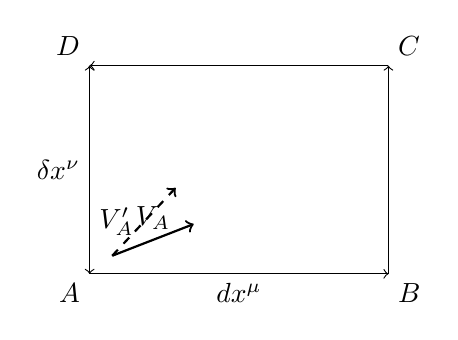
\begin{tikzpicture}[scale=1.15]
\draw[->] (0,0) -- (3.3,0) node[midway,below] {$dx^\mu$};
\draw[->] (0,0) -- (0,2.3) node[midway,left] {$\delta x^\nu$};
\draw[->] (3.3,0) -- (3.3,2.3);
\draw[->] (3.3,2.3) -- (0,2.3);
\draw[->] (0,2.3) -- (0,0);

\node[below left] at (0,0) {$A$};
\node[below right] at (3.3,0) {$B$};
\node[above right] at (3.3,2.3) {$C$};
\node[above left] at (0,2.3) {$D$};

\draw[->,thick] (0.25,0.2) -- (1.15,0.55) node[midway,above] {$V_A$};
\draw[->,thick,dashed] (0.25,0.2) -- (0.95,0.95) node[midway,left] {$V_A'$};
\end{tikzpicture}
\caption{Schematic reconstruction of the infinitesimal loop \(A\to B\to C\to D\to A\). The vector returns to the same point, but in a curved geometry it need not return with the same orientation.}
\end{figure}

Call the transported vector at the end of the loop \(V_A'\). We want the difference \(V_A-V_A'\). Susskind does not simply announce the answer. He manufactures it from a difference of differences:
\begin{equation}
\big[(V_C-V_D)-(V_B-V_A)\big]
-
\big[(V_C-V_B)-(V_D-V_A')\big]
=
V_A - V_A'.
\end{equation}
The point of this expression is that all the interior terms cancel. What is left is exactly the small mismatch produced by transporting around the loop.

Now, for infinitesimal displacements, these finite differences become derivatives. More precisely, because we are parallel transporting, they become \emph{covariant} derivatives. The first bracket corresponds to taking a covariant difference in the \(dx^\mu\) direction and then differentiating that difference in the \(\delta x^\nu\) direction. The second bracket does the same thing in the opposite order. Thus the loop mismatch is
\begin{equation}
\Delta V
=
\big(\nabla_\nu\nabla_\mu-\nabla_\mu\nabla_\nu\big)V\,\delta x^\nu dx^\mu
=
[\nabla_\nu,\nabla_\mu]V\,\delta x^\nu dx^\mu.
\end{equation}

This is the moment the lecture has been preparing. Curvature is the failure of two covariant derivatives to commute.

\subsection{Question \& Answer}

Why this particular combination of differences? Susskind's answer in the lecture is refreshingly direct: because he knows what he wants to get. The sign convention is engineered so that the intermediate vectors cancel and the only survivor is the mismatch between the initial vector and the transported one. Had we reversed the loop orientation, the same physics would come back with the opposite overall sign.

What actually goes to zero when the loop shrinks? Not the curvature tensor. What becomes small is the \emph{change in the vector}. The mismatch \(\Delta V\) is proportional to the area of the loop, so it is quadratic in the two small edge lengths. A student asks, quite reasonably, whether one should divide by the area and think of this as a mixed second derivative. Susskind resists that temptation. This is not the second derivative of some scalar function. It is a commutator of covariant derivatives acting on a vector.

Does the choice of plane matter? Only in the obvious way. Any two infinitesimal vectors determine a plane. The Riemann tensor is the same tensor regardless of the plane one chooses, but different choices of \(dx^\mu\) and \(\delta x^\nu\) pick out different components of it.

With the operator language in place, the derivation becomes short. Using
\[
\nabla_\mu=\partial_\mu+\Gamma_\mu,
\]
we expand
\begin{align}
[\nabla_\nu,\nabla_\mu]
&=
[\partial_\nu+\Gamma_\nu,\partial_\mu+\Gamma_\mu] \\
&=
[\partial_\nu,\partial_\mu]
+
[\partial_\nu,\Gamma_\mu]
-
[\partial_\mu,\Gamma_\nu]
+
[\Gamma_\nu,\Gamma_\mu].
\end{align}
The first term vanishes because ordinary partial derivatives commute:
\begin{equation}
[\partial_\nu,\partial_\mu]=0.
\end{equation}
The middle terms are exactly of the type handled by the commutator lemma, so they give derivatives of \(\Gamma\). The last term survives because the \(\Gamma_\mu\) are matrices and matrices need not commute. Therefore
\begin{equation}
[\nabla_\nu,\nabla_\mu]
=
\partial_\nu\Gamma_\mu
-
\partial_\mu\Gamma_\nu
+
\Gamma_\nu\Gamma_\mu
-
\Gamma_\mu\Gamma_\nu.
\end{equation}

Restoring the hidden matrix indices, we arrive at the standard component formula
\begin{equation}
R^\alpha{}_{\beta\mu\nu}
=
\partial_\mu \Gamma^\alpha{}_{\nu\beta}
-
\partial_\nu \Gamma^\alpha{}_{\mu\beta}
+
\Gamma^\alpha{}_{\mu\delta}\Gamma^\delta{}_{\nu\beta}
-
\Gamma^\alpha{}_{\nu\delta}\Gamma^\delta{}_{\mu\beta}.
\end{equation}
The change in the vector around the loop is then
\begin{equation}
\Delta V^\alpha
=
R^\alpha{}_{\beta\mu\nu}\,V^\beta\,\delta x^\nu dx^\mu.
\end{equation}

Susskind later compresses the whole construction into the elegant schematic statement
\begin{equation}
R_{\mu\nu}\sim[\nabla_\mu,\nabla_\nu],
\end{equation}
with the warning that the suppressed indices are matrix indices. One must not forget that the curvature is an operator acting on vectors.

\section{Symmetries, Contractions, and Lower-Rank Curvature}

Once the Riemann tensor is on the board, the lecture changes pace. We are no longer deriving it; we are reading structure off from it. Lower the first index with the metric and write the tensor as \(R_{\nu\mu\alpha\beta}\). In that form the lecture emphasizes the basic symmetry pattern:
\begin{equation}
R_{\nu\mu\alpha\beta}=-R_{\mu\nu\alpha\beta},
\qquad
R_{\nu\mu\alpha\beta}=-R_{\nu\mu\beta\alpha},
\qquad
R_{\nu\mu\alpha\beta}=R_{\alpha\beta\nu\mu}.
\end{equation}
The first antisymmetry is immediate from the commutator. The second is stated in the lecture and tied to the preservation of vector length under parallel transport. The third is the pair-exchange symmetry of the fully lowered tensor.

There is also a structural observation that matters later. The Christoffel symbols contain first derivatives of the metric. Therefore the Riemann tensor contains two kinds of terms: second derivatives of the metric and quadratic products of first derivatives. This is exactly the sort of object one expects to appear on the geometric side of a field equation.

\begin{figure}[htbp]
\centering

\includegraphics[width=0.55\textwidth]{lecture_08_figure_02.png}
\caption{Ricci-contraction notation on the board. The board isolates the contraction pattern itself; the exact raised and lowered placement is partly obscured, so we pair it with clean standard notation in the text.}
\end{figure}

Now the lecture asks a new question: what lower-rank tensors can we make from the Riemann tensor?

If we contract the antisymmetric pair \(\mu,\nu\) with the symmetric metric, we get zero:
\begin{equation}
g^{\mu\nu}R_{\mu\nu\alpha\beta}=0.
\end{equation}
The reason is simple and very much in the lecture's spirit: a symmetric object contracted with an antisymmetric one vanishes.

The same happens if we contract the antisymmetric pair \(\alpha,\beta\):
\begin{equation}
g^{\alpha\beta}R_{\mu\nu\alpha\beta}=0.
\end{equation}
So the interesting contraction must be a mixed one. In clean standard notation we define the Ricci tensor by
\begin{equation}
R_{\mu\nu}
=
R^\alpha{}_{\mu\alpha\nu}.
\end{equation}
Equivalently, with all indices lowered, one may write
\begin{equation}
R_{\mu\beta}
=
g^{\alpha\nu}R_{\nu\mu\alpha\beta},
\end{equation}
which is the contraction pattern the board image is hinting at.

The lecture then notes that \(R_{\mu\nu}\) is symmetric, again as a consequence of the symmetries of the Riemann tensor. Contracting once more gives the scalar curvature:
\begin{equation}
R=g^{\mu\nu}R_{\mu\nu}.
\end{equation}

Susskind is careful here not to let the scalar do more work than it should. If the curvature scalar is nonzero, the space is curved. But if it vanishes, that is not in general enough to guarantee flatness. The lecture mentions only the dimension-dependent facts it needs: in two dimensions the scalar already controls flatness, in three dimensions the Ricci tensor does, and in higher dimensions one must really look to the full Riemann tensor.

\paragraph{Intrinsic and extrinsic curvature.}
The lecture pauses here for an important warning. Curvature in this sense is intrinsic. A sheet of paper may be bent in an ambient three-dimensional space and still have zero intrinsic curvature. The Riemann tensor is not measuring how a space is embedded somewhere else. It measures what is felt by someone who lives and moves within the space itself.

\section{Slow Geodesics and the Newtonian Potential}

At this point the lecture makes a hard turn. We stop asking what curvature \emph{is}, and begin asking how general relativity reproduces Newtonian gravity in the regime where Newton should be right.

The equation of motion is the geodesic equation. Susskind phrases it first in words: the tangent vector is covariantly constant along the trajectory. In components,
\begin{equation}
\frac{d^2x^\mu}{d\tau^2}
+
\Gamma^\mu{}_{\sigma\lambda}
\frac{dx^\sigma}{d\tau}
\frac{dx^\lambda}{d\tau}
=
0,
\end{equation}
with proper time defined by
\begin{equation}
d\tau^2 = g_{\mu\nu}\,dx^\mu dx^\nu.
\end{equation}

Now we restrict attention to the Newtonian regime. There are really two assumptions. First, everything is moving slowly in some chosen frame. Second, the gravitational field is weak, so the metric differs only slightly from the Minkowski metric:
\begin{equation}
g_{\mu\nu}=\eta_{\mu\nu}+h_{\mu\nu},
\qquad
|h_{\mu\nu}|\ll 1.
\end{equation}
In that regime,
\begin{equation}
x^0=t\approx \tau,
\qquad
\frac{dx^0}{d\tau}\approx 1,
\qquad
\frac{dx^i}{d\tau}\ll 1.
\end{equation}
So for a spatial coordinate, say \(x\), the geodesic equation reduces to
\begin{equation}
\frac{d^2x}{dt^2}\approx -\Gamma^x{}_{00}.
\end{equation}
This is the first great simplification of the second half of the lecture: the Christoffel symbol with two zero indices is playing the role of the Newtonian gravitational field.

Let us expand it:
\begin{align}
\Gamma^x{}_{00}
&=
\frac12 g^{x\rho}
\left(
\partial_0 g_{\rho 0}
+
\partial_0 g_{0\rho}
-
\partial_\rho g_{00}
\right) \\
&\approx
\frac12 g^{xx}
\left(
2\,\partial_0 g_{x0}
-
\partial_x g_{00}
\right).
\end{align}
Now the lecture uses the slow-motion assumption once again. If the sources are moving slowly, the metric changes only slowly in time. Thus the time-derivative terms may be neglected, and \(g^{xx}\) may be replaced by \(\eta^{xx}=-1\) to the order we are keeping. Therefore the cleaned weak-field result is
\begin{equation}
\frac{d^2x}{dt^2}\approx -\frac12\,\frac{\partial g_{00}}{\partial x}.
\end{equation}

\begin{figure}[htbp]
\centering

\includegraphics[width=0.55\textwidth]{lecture_08_figure_03.png}
\caption{Newtonian acceleration and the boxed metric-potential relation on the board. The lecture is visibly unstable on signs here, but the boxed relation marks the intended conclusion.}
\end{figure}

Now we compare with Newtonian gravity, where the acceleration is
\begin{equation}
\frac{d^2x}{dt^2}=-\frac{\partial \phi}{\partial x}.
\end{equation}
Susskind is very candid here: he loses track of a sign on the board and says so. It is worth preserving that hesitation because it is part of the lecture's rhythm. The exact sign matters physically, but the structural conclusion does not depend on settling it on the spot. What survives the comparison is that \(g_{00}\) must be related to the Newtonian potential \(\phi\) by a factor of \(2\) and an additive constant:
\begin{equation}
g_{00}=2\phi+c.
\end{equation}
Far away from gravitating matter the metric must approach the Minkowski form, so eventually \(c=1\). But the lecture does not stop here to make that constant the center of attention. The important point is that the time-time component of the metric already knows about the Newtonian potential.

\section{Poisson's Equation and the Search for a Tensor Equation}

Having tied \(g_{00}\) to \(\phi\), the lecture goes back to Newton once more and asks about sources. What equation does the Newtonian potential satisfy?

The board presents this as a vertical progression: first the acceleration field, then its divergence law, then Poisson's equation.

\begin{figure}[htbp]
\centering

\includegraphics[width=0.52\textwidth]{lecture_08_figure_04.png}
\caption{Newtonian gravity equations for the potential. The board is arranged vertically, exactly as the lecture proceeds from acceleration field to divergence law to Poisson's equation.}
\end{figure}

The top line on the board is not perfectly legible, and the lecture itself is not steady on the associated sign convention. The stable mathematical content is the source law
\begin{equation}
\nabla\cdot A = -4\pi G\rho,
\end{equation}
together with the corresponding Poisson equation
\begin{equation}
\nabla^2\phi = 4\pi G\rho.
\end{equation}
The Laplacian here is simply
\begin{equation}
\nabla^2\phi
=
\frac{\partial^2\phi}{\partial x^2}
+
\frac{\partial^2\phi}{\partial y^2}
+
\frac{\partial^2\phi}{\partial z^2}.
\end{equation}

Now the lecture makes the relativistic identification. In units with \(c=1\), mass density is energy density, and energy density is the \(00\)-component of the energy-momentum tensor. That is the unmistakable point of the surrounding discussion, even though this stretch of the spoken record is rough. Therefore
\begin{equation}
\rho \leftrightarrow T^{00},
\qquad
\nabla^2\phi = 4\pi G T^{00}.
\end{equation}
Using the earlier weak-field relation \(\phi=\tfrac12 g_{00}\), we obtain
\begin{equation}
\nabla^2 g_{00}=8\pi G T^{00}.
\end{equation}

\begin{figure}[htbp]
\centering

\includegraphics[width=0.60\textwidth]{lecture_08_figure_05.png}
\caption{Poisson equation rewritten with \(T^{00}\). This is the board moment where the source term is explicitly reinterpreted as the energy-density entry of the stress-energy tensor.}
\end{figure}

This is the first place where the lecture begins to see a real geometric field equation trying to emerge. A component of the metric is being controlled by a component of the energy-momentum tensor.

\subsection{Question \& Answer}

What is wrong with the equation
\[
\nabla^2 g_{00}=8\pi G T^{00}?
\]
The answer is not that it is false. On the contrary, it is exactly the right weak-field equation in the slow-moving frame in which it was derived. The problem is that it is not yet a tensor equation. It singles out one component, \(g_{00}\), in one special frame. General relativity cannot stop there. The whole point of tensors is that if an equation is true in one frame, it is true in every frame.

This objection is the final tension of the lecture, and it is essential not to flatten it away. The lecture does not end with Einstein's equation; it ends with the need for Einstein's equation.

\begin{figure}[htbp]
\centering

\includegraphics[width=0.72\textwidth]{lecture_08_figure_06.png}
\caption{Weak-field equation beside the first stress-energy entries. The split board shows the transition from scalar weak-field reasoning to the search for a genuine tensor equation.}
\end{figure}

The right-hand side is already a piece of a tensor. The board indicates this by sketching the beginning of the energy-momentum matrix and, beside it, by expanding the Laplacian into coordinate derivatives. Schematically,
\begin{equation}
T^{\mu\nu}\sim
\left(
\begin{array}{ccc}
T^{00} & T^{01} & \cdots \\
T^{10} & T^{11} & \cdots \\
\vdots & \vdots & \ddots
\end{array}
\right).
\end{equation}
So the left-hand side must also be a two-index tensor, built only from the metric and its derivatives, and in the Newtonian limit its \(00\)-component must reduce to the weak-field equation above.

By now the lecture has already prepared the answer to the preparatory question: what geometric tensors with two indices can be made from the metric and its second derivatives? The natural possibilities are \(R_{\mu\nu}\) and \(g_{\mu\nu}R\). Therefore the most general candidate at this stage is
\begin{equation}
A\,R_{\mu\nu}+B\,g_{\mu\nu}R = 8\pi G\,T_{\mu\nu},
\end{equation}
where \(A\) and \(B\) are numerical coefficients.

Susskind even gives away, almost mischievously, that the numbers will turn out to be \(1\) and \(-\tfrac12\). But he does not derive that here, and we should not pretend that he has. The lecture ends exactly where it wants to end: with the target set, the Newtonian limit understood, and the Einstein tensor still to be found in the next step of the story.

\section{Summary}

The lecture begins with curvature in its geometric form: a vector carried around a small loop fails to return to itself. To derive the corresponding tensor cleanly, Susskind shifts into operator language and treats the covariant derivative as ``ordinary derivative plus a matrix.'' The commutator of two such derivatives gives the infinitesimal loop mismatch, and that commutator is the Riemann tensor.

Once the Riemann tensor is in hand, the lecture pauses to read off its symmetries and to see what contractions survive. That guided bookkeeping leads to the Ricci tensor and the scalar curvature. The second half then turns toward physics. In the weak-field, slow-motion limit, the geodesic equation reduces to Newtonian acceleration, and the time-time component of the metric becomes tied to the Newtonian potential. Poisson's equation then turns into a weak-field relation between \(g_{00}\) and \(T^{00}\).

The lecture ends, not with a finished field equation, but with the right question: what two-index tensor made from the metric and its derivatives reduces to that weak-field equation and therefore deserves to stand on the left-hand side of the full gravitational theory?